\section{Le terminal virtuelle}

\begin{frame}

	\begin{itemize}[<+->]
		\item L'apparition des ordinateurs personnels
			\begin{figure}
				\centering
				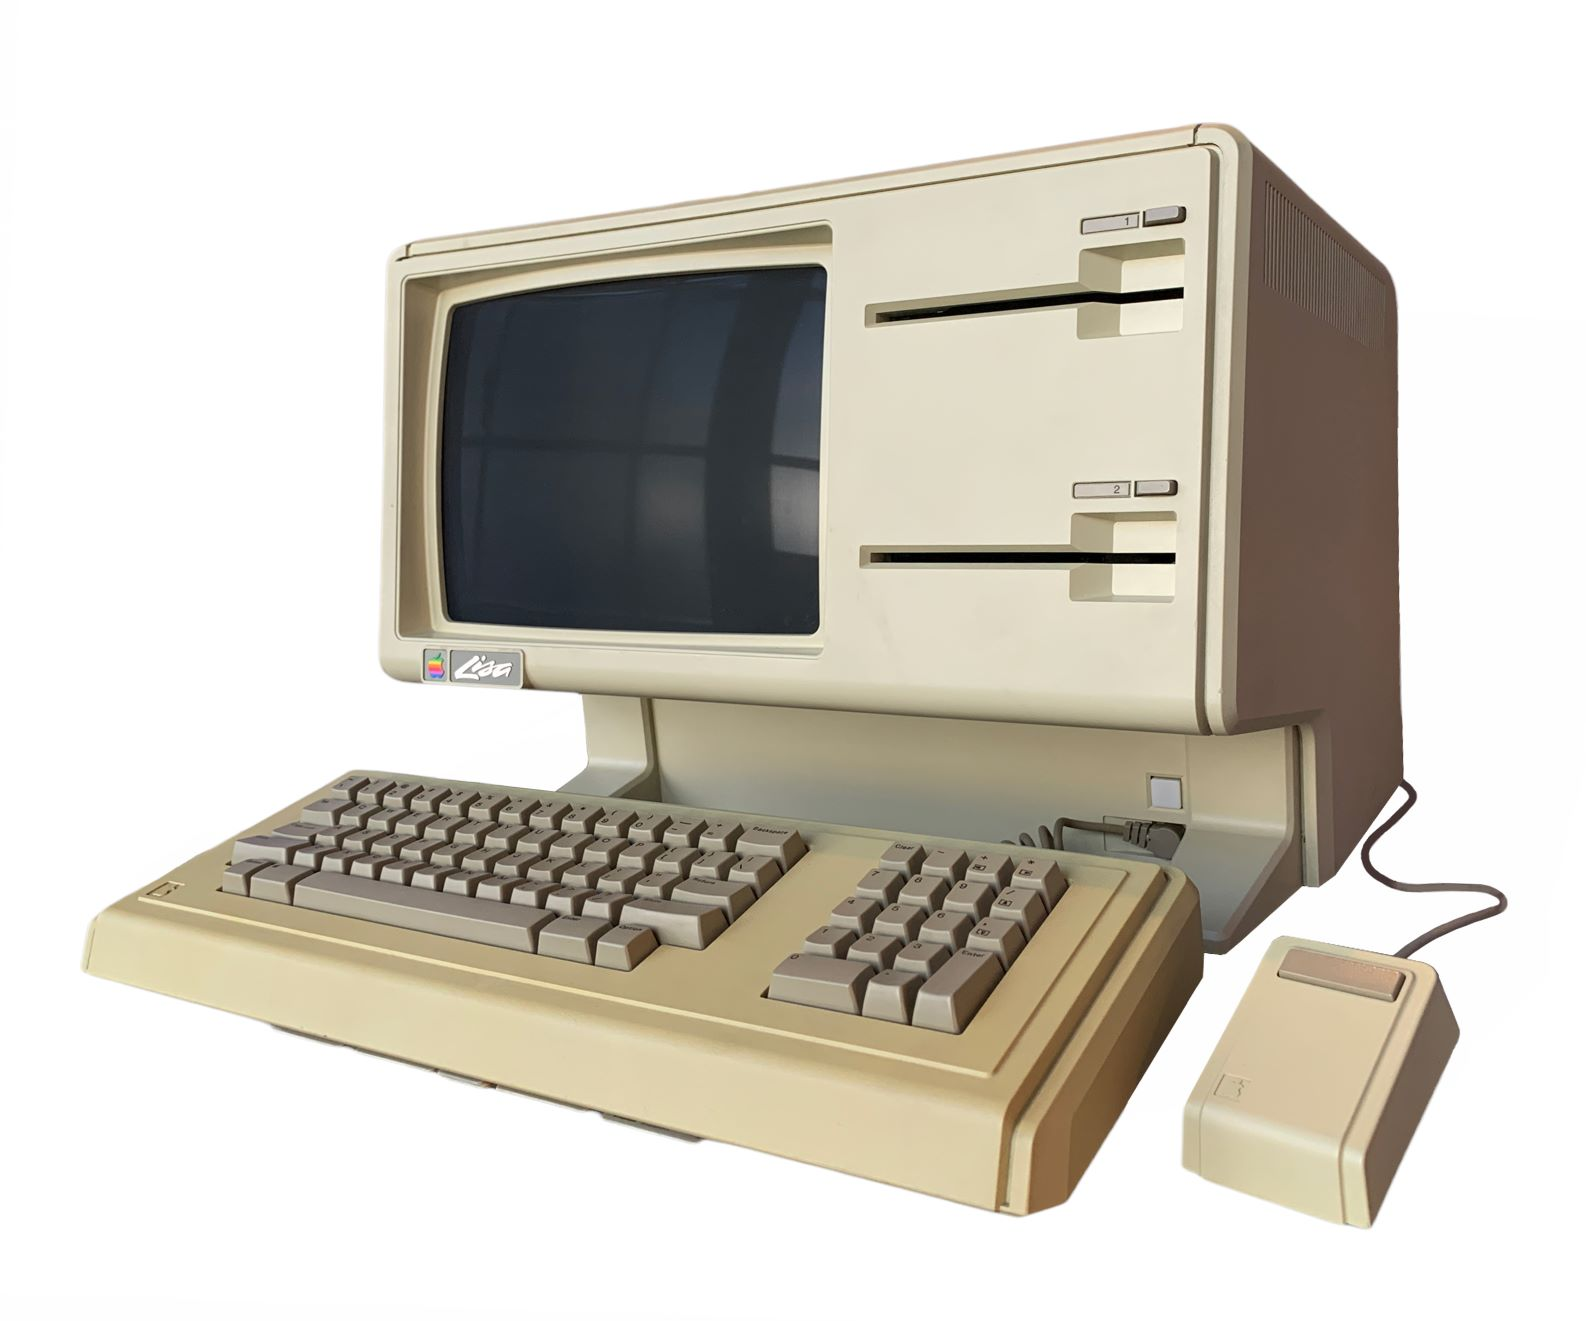
\includegraphics[width=4cm]{images/apple_lisa.jpg}
				\caption{Un ordinateur personnel surnommé "Lisa" créé par Apple.}
			\end{figure}

		\item Il n'était plus nécessaire d'utiliser l'unité centrale pour effectuer des calculs informatiques

		\item Les terminaux physiques sont utilisés de moins en moins
	\end{itemize}

\end{frame}

\begin{frame}

	\begin{itemize}[<+->]
		\item Utilisation d'interfaces en mode texte sur les ordinateurs personnels
		
		\item Quelques années plus tard, l'avènement des terminaux virtuels
		
		\item Possibilité d'ouvrir plusieurs sessions sur les consoles virtuelles
	\end{itemize}

\end{frame}

\begin{frame}

	\begin{itemize}[<+->]
		\item Offre une interface textuelle pour \textbf{interagir} avec le système d'exploitation
			\begin{figure}
				\centering
				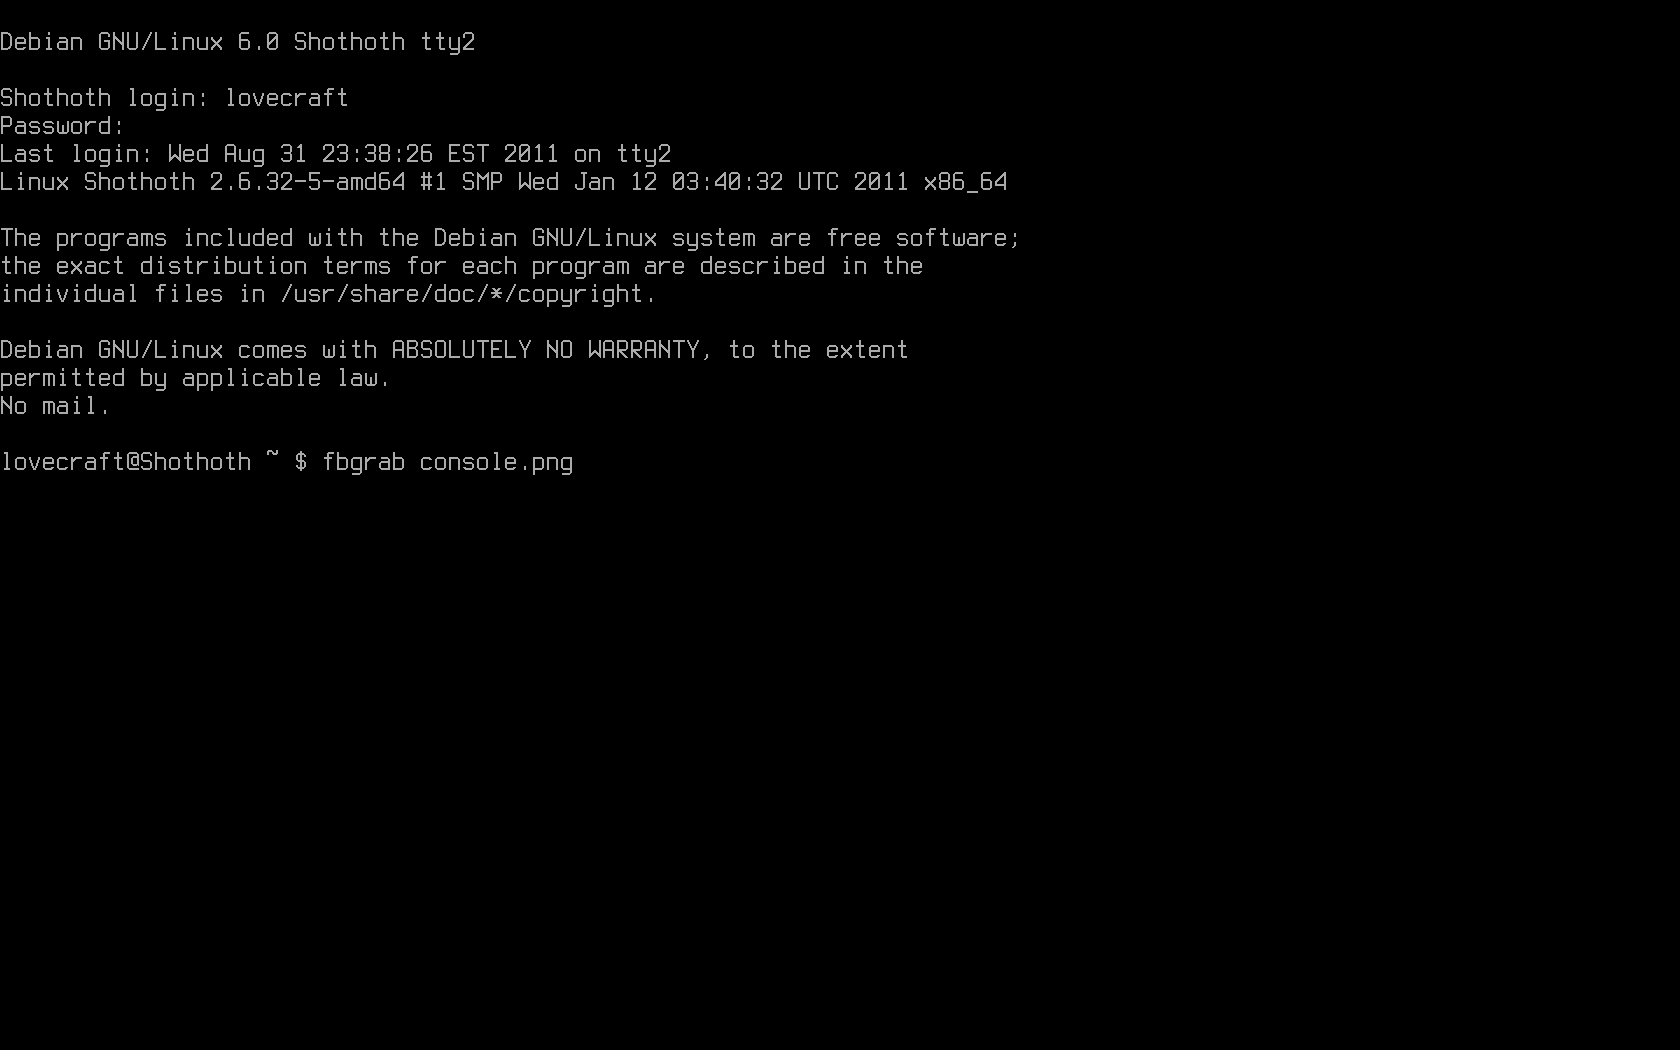
\includegraphics[width=5cm]{images/virtual_console.png}
				\caption{L'affichage d'une console virtuelle}
			\end{figure}
		\item Reçoit les entrées de l'utilisateur et affiche les résultats à l'écran

		\item Fonctionne de manière similaire à un \textbf{terminal physique}

	\end{itemize}

\end{frame}

\begin{frame}

	\begin{itemize}[<+->]

		\item Un répertoire spécial représentant les périphériques sous forme de fichiers

		\item Le répertoire \textbf{/dev} sur Linux/Unix
               
		\item Deux types de périphériques : \textit{caractère} \& \textit{bloc}
               
		\item Un terminal virtuel est un périphérique de type \textit{caractère}

	\end{itemize}

	\begin{block}{Quel est la différence}
		\begin{itemize}
			\item Un périphérique de type \textit{caractère} envoie \& reçoit des données sous forme de bytes
			\item Un périphétique de type \textit{block} envoie \& reçoit des données sous forme de blocs de bytes
		\end{itemize}
	\end{block}

\end{frame}

\begin{frame}	
	\begin{itemize}[<+->]
		\item Pour chaque périphérique, il y a un \textit{pilote}
        
		\item Un \textit{pilote} est essentiel pour le bon fonctionnement du périphérique
        
		\item Le terminal virtuel possède lui aussi un pilote appelé : \textbf{pilote de terminal}
	\end{itemize}

\end{frame}

\begin{frame}
	\begin{itemize}[<+->]
		\item Le \textbf{pilote de terminal} possède 2 tampons pour stocker des données

		\item Un tampon d'entrée appelé: \textit{input buffer}

		\item Un tampon de sortie appelé: \textit{output buffer}

	\end{itemize}

	\begin{block}{Une taille fixe pour le tampon d'entrée}
		Le tampon d'entrée possède une taille fixe définie par l'OS, généralement de \textit{4096 octets}. Il est impossible d'ajouter des données au-delà de cette taille.
	\end{block}
\end{frame}

\begin{frame}
	\begin{itemize}[<+->]
		\item Les entrées au clavier sont réceptionnées par le pilote du clavier et renvoyées pour traitement à l'OS
		\item Le \textbf{pilote de terminal} stocke les données reçues dans un tampon de taille fixe
		\item Les données sont traitées pour détecter tout caractère spécial

\item Le processus \textit{lecteur} effectue une lecture sur le tampon pour récupérer les données

\item Les données venant du processus \textit{lecteur} sont stockées dans un autre tampon
	\end{itemize}
\end{frame}

\begin{frame}
	\begin{itemize}[<+->]
		\item Le \textbf{pilote de terminal} peut être en mode \textit{canonique} ou \textit{non-canonique}
			\begin{figure}
				\centering
				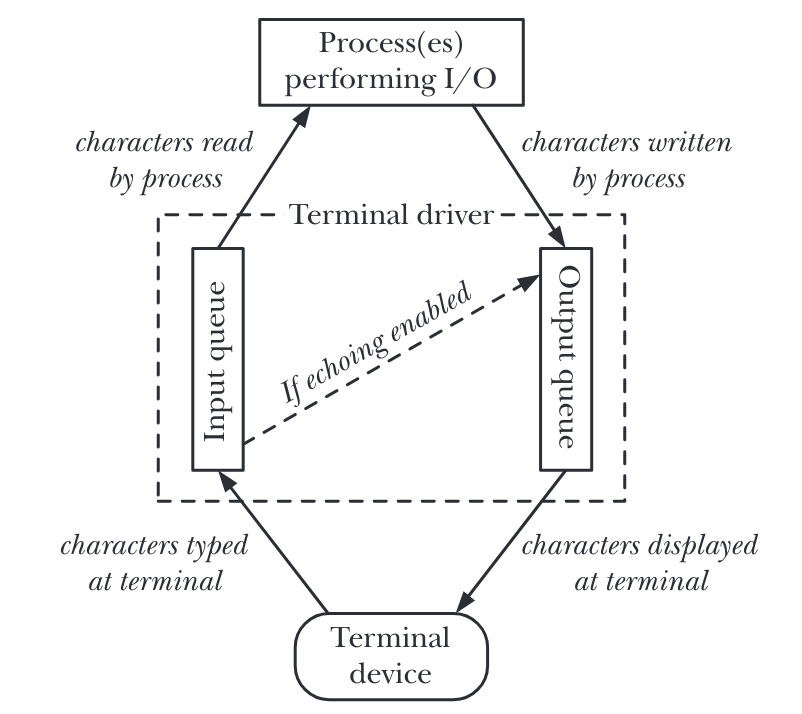
\includegraphics[width=4cm]{images/input_output_queue.png}
				\caption{Le schèma représentant les 2 tampons}
			\end{figure}
		\item En mode \textit{canonique}, les données sont stockées par ligne
		
		\item En mode \textit{non-canonique}, les données sont stockées par octets
	\end{itemize}
\end{frame}

\begin{frame}
	\begin{itemize}[<+->]
		\item Prise en charge des caractères spéciaux en mode canonique

		\item La touche \textit{Entrée} génère un caractère spécial \textbf{EOF}

		\item Des combinaisons de touches génèrent aussi des caractères spéciaux

	\end{itemize}

	\begin{examples}
		\begin{itemize}[<+->]
			\item Une fois que les données sont entrées par l'utilisateur et que celui-ci presse la touche \textit{Entrée}, un caractère spécial \textbf{EOF} à la fin de la ligne avertit le processus \textit{lecteur} qu'une lecture peut être effectuée.
			\item Le fait d'appuyer sur une combinaison de touches \textit{CTRL+C} génère un signal \textit{INTR} sur tous les processus tournant en \textbf{foreground}.
		\end{itemize}
	\end{examples}
\end{frame}

\begin{frame}
	\begin{itemize}[<+->]
		\item En mode non-canonique, les caractères spéciaux ne sont pas pris en compte.
		
		\item Le \textit{line editing} n'est également pas possible

		\item Le processus \textit{lecteur} lit directement les octets stockés dans le tampon.
	\end{itemize}
\end{frame}
